% TUTTO IL PDF %
\section{Cryptography at work: PKI and TLS}
    \subsection{Recall of PKC}
    The Public Key Cryptography pros
    \begin{itemize}
        \item Private key is only known by the owner
        \item Confidentiality by encrypting with Receiver's Public Key
        \item Non repudiation by encrypting with Sender's Private Key
    \end{itemize}
    The cons are
    \begin{itemize}
        \item Algorithms are 2-3 orders of magnitude slower than those for symmetric encryption
        \item How are Public keys made available to the other people
        \item There is still a big problem of Authentication: who ensures that the owner of a key pair is really the person whose real life name is "Alice".
    \end{itemize}  
    So in reality the \textbf{non repudiation} cannot be proven. A mitigation for this is a \textbf{Digital signature}, a data item that vouches the origin and the integrity of a message. 
    
    \begin{figure}[h!]
        \centering
        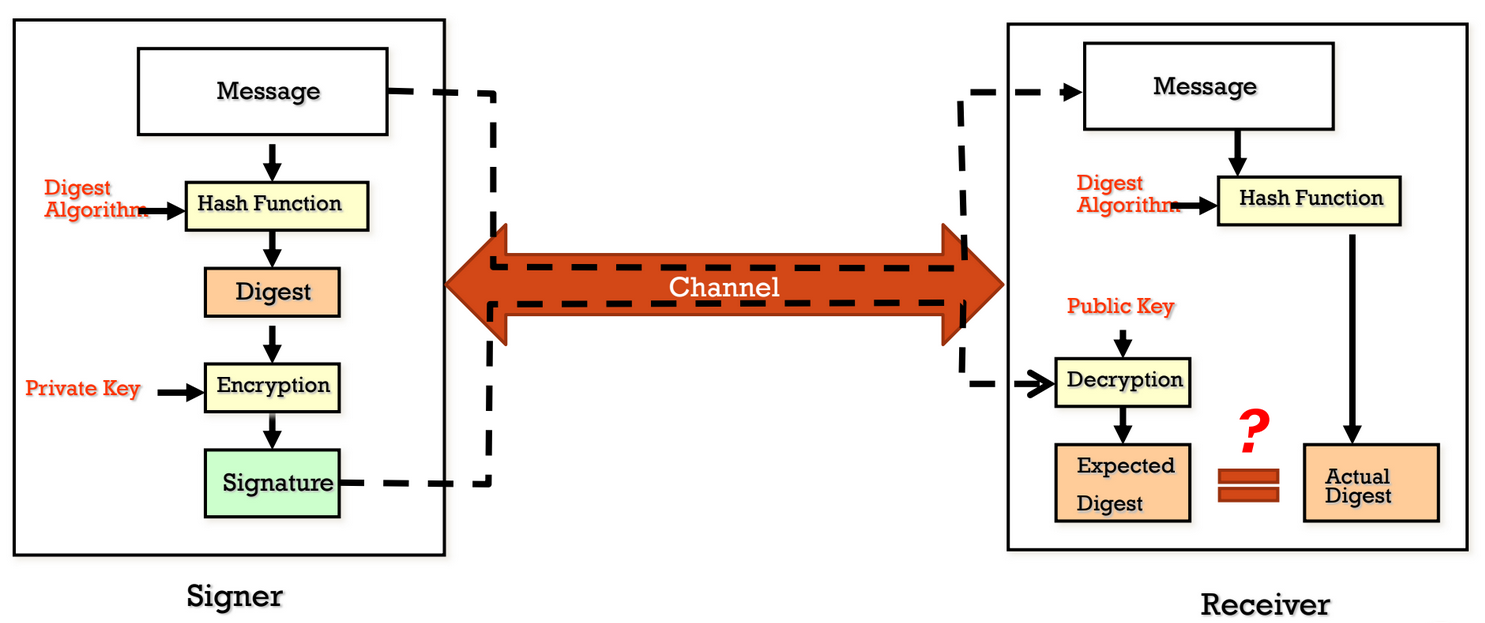
\includegraphics[scale=0.3]{images/PKCcomm.png}
    \end{figure}
    
    \FloatBarrier
    
    The problem now is who guarantees that the one using the key is entitled to do so?
    
    \subsection{Public Key Infrastructure}
    The main requirement on public key is to be authentically bound to the identity of the party controlling the corresponding private key, another requirement is that parties relying on the correctness binding between public keys and corresponding party identities can be assured that the binding is still valid. Statisfying these two requirements is typically done by setting up a \textbf{Public Key Infrastructure}.
    
    \myparagraph{Digital Certificates}
    The initial proposal was to store the certificates as a bulletin boards so the public key and identities are listed. This is non scalable and inflexible approach adopted in mobile and Internet of Things applications is to \textbf{hardcode} the public key in the software of the party. 
    
    A widely adopted solution is the use of \textbf{digital certificates}, are digital objects containing data including the identity and the public key that are signed by a Trusted Third Party \textbf{(TTP)}, it bind an entity's Public Key and one or more attributes concerning its Identity (entity can be a person, an hardware component, a service ...). A Digital Certificate is issued and signed by a TTP that is also called Certificate Authority \textbf{(CA)}. The standard for certificates is the X.509, the validity of this certificate last for 6/12 month and at the end has the CA digital signature to prove the authenticity.
    
    \subsection{Public Key Infrastructure}
    A Public Key Infrastructure \textbf{(PKI)} is an arrangement that binds public keys with respective identities of entities. The binding is established through a process if registration and issuance of certificates at and by a CA. The PKI role that assures valid and correct registration is called a Registration Authority \textbf{(RA)}. A third-party Validation Authority \textbf{(VA)} can provide an entity information on behalf the CA.
    
    So a PKI is a system that provides for a TTP to vouch for user identities and allows binding of public keys to subjects. Components:
    \begin{itemize}
        \item root Certificate Authority, the most significant element in the CA hierarchy
        \item Registration Authority that verifies information in a certificate request
        \item Cryptographic Practices Statement (CPS)
        \item Certificate Revocation List (CRL)
    \end{itemize}
    
    \begin{figure}[h!]
        \centering
        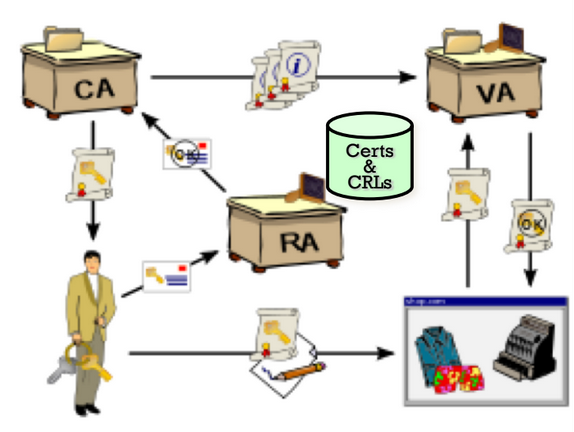
\includegraphics[scale=0.3]{images/PKI.png}
        \caption{The PKI infrastructure}
        \label{fig:pki}
    \end{figure}
    
    \FloatBarrier
    